\documentclass[11pt]{beamer}
% Packages
\usepackage{beamer-german}


% Title etc.
\title{Werte \& Wertewandel}
\subtitle{Analyse politischer Unterstützung in der quantitativen Forschungspraxis}
\date{21. Januar 2022}
\author{B. Philipp Kleer}
\institute{Institut für Politikwissenschaft | Justus-Liebig-Universität Gießen}

\setbeamerfont{itemize/enumerate body}{size = \small}
\setbeamerfont{itemize/enumerate subbody}{size = \footnotesize}
\setbeamerfont{itemize/enumerate subsubbody}{size = \scriptsize}

% Datumspaket
\usepackage[german]{isodate}

% Table packages
\usepackage{booktabs}
\usepackage{longtable}

\addbibresource{lit-s9.bib}

\begin{document}

\begin{frame}
	\maketitle
\end{frame}


\begin{frame}[t]{Präsentationen}

% Hier noch Präsentationen und Datum einfügen
	\begin{table}
		\begin{tabular}{m{0.15\textwidth} >{\centering} m{0.1\textwidth} >{\centering} m{0.3\textwidth}  >{\centering\arraybackslash} m{0.3\textwidth}}
			\toprule[2pt]
			\textbf{Datum} & \textbf{Gruppe} & \textbf{Wer?} & \textbf{Feedback}\\
			\midrule
			18.02.2022 & 1 & Wer & ...\\
			\midrule
			18.02.2022 & 2 & Wer & ...\\
			\midrule
			18.02.2022 & 3 & Wer & ...\\
			\midrule
			18.02.2022 & 4 & Wer & ...\\
			\midrule
			18.02.2022 & 5 & Wer & ...\\
			\midrule
			18.02.2022 & 5 & Wer & ...\\
			\bottomrule[2pt]
		\end{tabular}
	\end{table}
% m => horizontal zentriert in Zeile
% p => horizontal top aligned
% b => horizontal bottom aligned
%>{\raggedright} -> rechts aligned
% >{\raggedleft} -> links aligned (default}
% for footnoes: \footnote or footnotemark or footnotetext
\end{frame}

\begin{frame}{Feedback}
	\shine{Ziel}: Klären offener Fragen, Erkennen möglicher Fallstricke, Unterstützen bei Projekten

	\begin{itemize}
		\item dazu: aufmerksam Materialien vorher anschauen und aufmerksam zuhören
		\item Feedback wird nicht nur mündlich gegeben, sondern auch schriftlich (Stichpunkte/-sätze reichen, keine formale Form)
			\begin{itemize}
				\item[$\Rightarrow$] Upload in ILIAS
			\end{itemize}
		\item Präsentierende: 3 Tage vor Präsentation Upload der Präsentation und/oder Handout $\Rightarrow$ Donnerstag 23:59h vor Präsentation ist Deadline!
			\begin{itemize}
				\item 10 Minuten Präsentation, 20 Minuten Diskussion	
			\end{itemize}
	\end{itemize}
\end{frame}

\begin{frame}{Textexperten}
	\begin{itemize}
		\item \cite{Welzel2013}: 
		\item \cite{Inglehart2010}: 
		\item \cite{Scherer2020}:
		\item \cite{Welzel2009}:
	\end{itemize}
\end{frame}

\begin{frame}{Postmaterialismus / Silent Revolution \parencite{Inglehart1977}}
	\begin{itemize}
		\item „The values of Western publix have been shifting from an overwhelming emphasis on material well-being and physical security toward greater emphasis on the quality of life.“ \parencite[1]{Inglehart1977}
		\item seit den 1960er Jahren Wertewandel in westlichen Industriegesellschaften beobachtbar
		\item Wechselwirkung mit Individualisierungs-, Modernisierungsprozessen (Wirtschaftswachstum, Wohlfahrtsstaat, Bildungsexpansion)
		\item[$\Rightarrow$] Wandel von materialistischen zu postmaterialistischen Werten
	\end{itemize}		

\end{frame}

\begin{frame}{Postmaterialismus / Silent Revolution \parencite{Inglehart1977}}
	\shine{Annahmen:}
	\begin{itemize}
		\item zentrale Rolle von Wertorientierungen im individuellen Überzeugungssystem („belief system“)
		\item Mangelhypothese
			\begin{itemize}
				\item Hierarchie menschlicher Bedürfnisse \parencite{Maslow1943}
			\end{itemize}
		\item Sozialisationshypothese
			\begin{itemize}
				\item Wertorientierungen werden in formativer Phase erworben
			\end{itemize}						
	\end{itemize}		
\end{frame}

\begin{frame}{Human Empowerment \parencite{Welzel2013}}
	\begin{figure}[ht]
		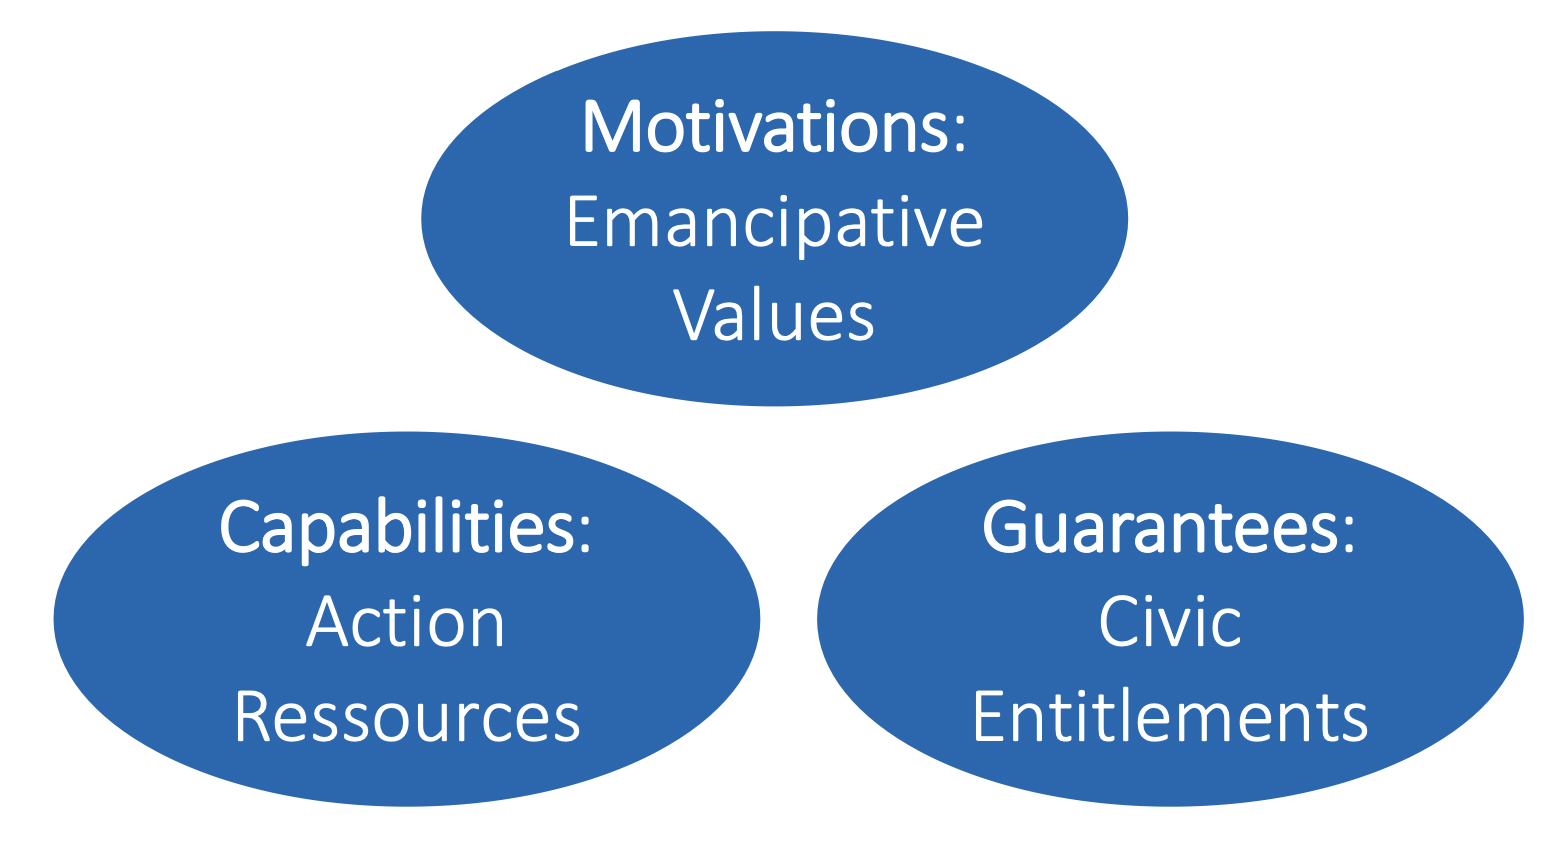
\includegraphics[width=\textwidth]{pics/s9-1.png}
		\caption{\textbf{Theoretischer Überblick}}
	\end{figure}
\end{frame}

\begin{frame}{Human Empowerment}
	\begin{itemize}
		\item Demokratisierung und Demokratie-Stabilität ist durch weiten Anstieg der Präferenz individueller Freiheitsrechte gekennzeichnet \parencite{Welzel2013}
		\item individuelle Freiheitsrechte sind Ausdruck intrinsischer Motivation für demokratische Prinzipien \parencite{Welzel2013}
		\item Empirisch überprüfbar gestaltet als emancipative values \parencite{Welzel2013}
		\begin{itemize}
			\item Gesellschaften mit höherer “Zustimmung” erreichen eher höheres Level an
	Demokratie \parencite[398]{Welzel2007}
		\end{itemize}
	\end{itemize}
\end{frame}

\begin{frame}{Human Empowerment \parencite[71]{Welzel2013}}
	\begin{columns}
		\begin{column}{0.3\textwidth}
			\begin{figure}[ht]
				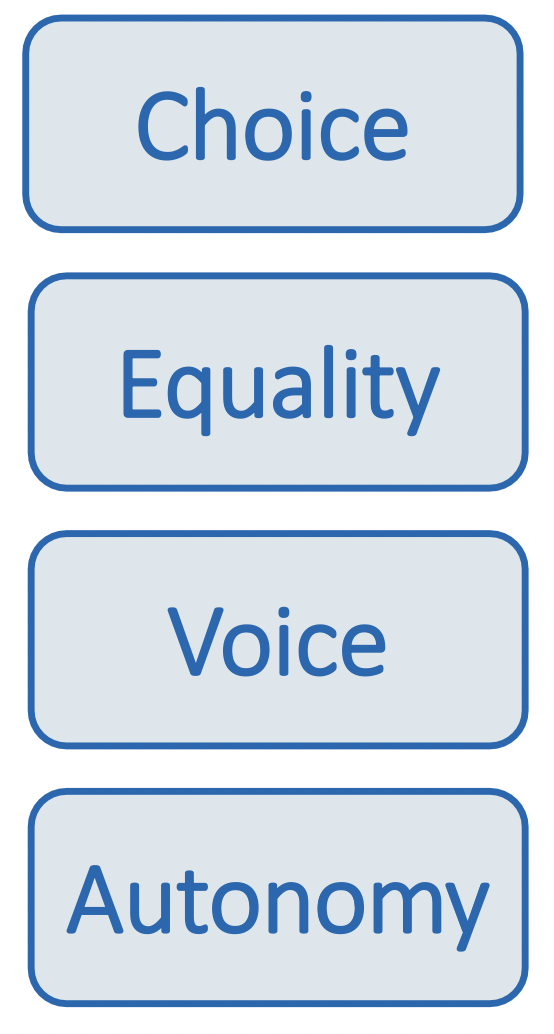
\includegraphics[width=\textwidth]{pics/s9-2.png}
			\end{figure}
		\end{column}
		\begin{column}{0.7\textwidth}
			\begin{itemize}
				\item Tolerance of Abortion, Divorce and Homosexuality
				\item[]
				\item Women‘s equality (Politic, Education, Job)
				\item[]
				\item Priority more to say (local/national)
				\item Freedom of Speech
				\item Independence a desired quality
				\item Obedience not a desired quality
				\item Imagination a desired quality
			\end{itemize}
		\end{column}
	\end{columns}

\end{frame}

\begin{frame}{\cite{Scherer2020}}
	\begin{itemize}
		\item Werte sind grundlegende Orientierungen, die Menschen dabei behilflich sind, aus einer potenziell unbegrenzten Zahl moglicher Handlungen und denkbarer Einstellungen zu wählen \parencite[210]{Scherer2020}
		\item Schlüsselstellung innerhalb des hierarchisch organisierten menschlichen Überzeugungssystems
		\item Vergleichsweise stabil gegenüber Einstellungen und Meinungen 
		\item Ausbildung in frühen Jahren
		\item Es gibt Zielkonflikte zwischen Werten (Hierarchisierung notwendig) 
		\item terminal vs. instrumentell
	\end{itemize}
\end{frame}

\begin{frame}{\cite{Welzel2009}}
	\begin{itemize}
		\item Werte sind dauerhaft verinnerlichte Zielmaßstäbe menschlichen Handelns
		\item Unterschied zu Normen: Normen werden sanktioniert
		\item Werteorientierung: verinnerlichte Werte
		\item Mikro: Menschen definieren sich über individuelle Werteprofile
		\item Makro: Kultur definiert sich über kollektiv vorherrschende Werteprofile
		\item Rating vs. Ranking (Wertehierarchie vs. Wertesynthese-Ansatz)
	\end{itemize}
\end{frame}

\begin{frame}{Praxisaufgabe}
	\shine{Datensatz}: World Values Survey, Round 6

	\begin{nolist}
		\item Finde heraus, aus welchem Land oder aus welchen Ländern das Subset besteht.
		\item Suche Items die auf das theoretische Konzept Choice passen.
		\item Überprüfe den Zusammenhang zwischen diesen Variablen.
	\end{nolist}

	\shine{Zeit}: 30 Minuten.
\end{frame}

\renewcommand*{\bibfont}{\scriptsize}

\begin{frame}[allowframebreaks]{Literatur}
	\nocite{*}
	\printbibliography[heading = none]
\end{frame}



\section{Mittagspause! \\ Wir treffen uns um 12:30 Uhr wieder.}

\end{document}
